\documentclass[a4paper, 12pt]{scrartcl}
\usepackage[ngerman]{babel}
\usepackage[utf8]{inputenc}
\usepackage[T1]{fontenc}
\usepackage{lmodern}

\linespread{1.2}
\parindent0cm
\usepackage{graphicx}
\usepackage{hyperref}
\usepackage{float}
\usepackage{tabularx}
\usepackage{multicol}
\usepackage{units}
\usepackage{mathtools}
\usepackage{subcaption}

\usepackage{listings}
\usepackage{color}
\usepackage{geometry}
	\geometry{a4paper, top=25mm, left=20mm, right=20mm, bottom=30mm, headsep=10mm, footskip=12mm}
\usepackage{amssymb}
	

\lstset{literate=%
	{Ö}{{\"O}}1
	{Ä}{{\"A}}1
	{Ü}{{\"U}}1
	{ü}{{\"u}}1
	{ä}{{\"a}}1
	{ö}{{\"o}}1
	{█}{{$\blacksquare$}}1
	{~}{{\textasciitilde}}1
}

\definecolor{mygreen}{rgb}{0,0.6,0}
\definecolor{mygray}{rgb}{0.5,0.5,0.5}
\definecolor{mymauve}{rgb}{0.58,0,0.82}
\definecolor{deepred}{rgb}{0.6,0,0}

\lstset{ %
	backgroundcolor=\color{white},   % choose the background color; you must add \usepackage{color} or \usepackage{xcolor}; should come as last argument
	basicstyle=\scriptsize,          % the size of the fonts that are used for the code
	breakatwhitespace=false,         % sets if automatic breaks should only happen at whitespace
	breaklines=true,                 % sets automatic line breaking
	captionpos=b,                    % sets the caption-position to bottom
	commentstyle=\color{mygreen},    % comment style
	deletekeywords={...},            % if you want to delete keywords from the given language
	escapeinside={\%*}{*)},          % if you want to add LaTeX within your code
	extendedchars=true,              % lets you use non-ASCII characters; for 8-bits encodings only, does not work with UTF-8
	frame=single,	                 % adds a frame around the code
	keepspaces=true,                 % keeps spaces in text, useful for keeping indentation of code (possibly needs columns=flexible)
	keywordstyle=\color{blue},       % keyword style
	language=Python,                 % the language of the code
	morekeywords={*,...},            % if you want to add more keywords to the set
	emph={makevideo,checkgreen,checkblue,lenken,line,linienfahren,main},
	emphstyle=\color{deepred},
	numbers=left,                    % where to put the line-numbers; possible values are (none, left, right)
	numbersep=5pt,                   % how far the line-numbers are from the code
	numberstyle=\tiny\color{mygray}, % the style that is used for the line-numbers
	rulecolor=\color{black},         % if not set, the frame-color may be changed on line-breaks within not-black text (e.g. comments (green here))
	showspaces=false,                % show spaces everywhere adding particular underscores; it overrides 'showstringspaces'
	showstringspaces=false,          % underline spaces within strings only
	showtabs=false,                  % show tabs within strings adding particular underscores
	stepnumber=2,                    % the step between two line-numbers. If it's 1, each line will be numbered
	stringstyle=\color{mymauve},     % string literal style
	tabsize=2,	                     % sets default tabsize to 2 spaces
	title=\lstname                   % show the filename of files included with \lstinputlisting; also try caption instead of title
}
 
\begin{document}
	\thispagestyle{empty}
	\begin{flushright}
		
\includegraphics[width=5cm]{HAW_Logo.eps}
	\end{flushright}
	Hochschule für Angewandte Wissenschaften Hamburg\\
	Fakultät Design, Medien und Information\\
	Department Medientechnik\\[1ex]
	IT-Systeme\\
	Prof. Dr. Torsten Edeler
	
	\vspace{1cm}
	\begin{center}
		\large{Projektbericht}\\
		\LARGE{Raspberry Car -- Team II}
		
		\vspace{2ex}
		\large{	Jörn Kogerup\\
				Darius Weiberg\\
				Mirco Hülsemann}
		
		\vspace{2ex}
		\large{12. Februar 2018}
		
	\end{center}

\newpage
\tableofcontents
\newpage

\section{Einleitung}

Dieser Projektbericht dient der Dokumentation des Projekts “Entwicklung eines selbstfahrenden Autos” im Modul IT-Systeme des Studiengangs Medientechnik an der HAW Hamburg im Wintersemester 2017/18.\\

Autonomes Fahren ist derzeit ein großes und hochaktuelles Forschungsthema vieler Universitäten, IT-Unternehmen und Automobilhersteller. Mit Hochdruck arbeiten Unternehmen wie Tesla, General Motors oder Waymo zusammen mit IT-Firmen wie Intel und Google daran, selbstfahrende Autos für die breite Masse verfügbar zu machen.

Aufgrund der aktuellen Relevanz und der Tatsache, dass ein selbstfahrendes Auto die ideale Verkörperung eines informationstechnischen Systems ist, ist dieses Thema als Projekt für die Veranstaltung “IT-Systeme” im Wintersemester 2017/2018 auserwählt worden.\\

Der vorliegende Abschlussbericht enthält Erläuterungen zum Projektziel, zum Projektumfeld sowie zu den gegebenen technischen Rahmenbedingungen. Es wird das technische Konzept zur Erreichung des Projektziels vorgestellt sowie die einzelnen Schritte des Entwicklungsprozesses dokumentiert und erläutert. Der gesamte Code sowie Bilder sind im Anhang des Dokuments zu finden.

\section{Projektvorstellung}

Im Rahmen der Vorlesung IT-Systeme (6. Semester des Studiengangs Medientechnik) sollen die Studenten/Studentinnen in kleinen Gruppen ein autonomes Modellbau-Auto entwickeln, welches in der Lage sein soll, mithilfe von Sensoren und Kameras selbstständig eine vorher definierte “Rennstrecke” abzufahren. Die Aufgaben der Studenten umfassen dabei:


\begin{itemize}
	\item eine konzeptionelle Planung zur Umsetzung des Projekts
	\item die Konstruktion des Modellbau-Autos (dabei wird ein Bausatz verwendet) sowie der Rennstrecke
	\item die Auseinandersetzung mit der Funktionsweise der elektrischen Komponenten
	\item die Verschaltung der elektrischen Komponenten
	\item Programmierung und Implementierung des Steuer-Codes auf einem Raspberry Pi
\end{itemize}


Als zeitlicher Rahmen ist ein Semester vorgesehen. Pro Woche gibt es eine 3-stündige Einheit, in der die Studenten unter Betreuung am Projekt weiterarbeiten können. Es ist jedoch auch möglich, außerhalb dieser Einheit am Projekt weiterzuarbeiten.

Es gibt zudem zwei “Challenge”-Termine im Semester, zu welchen bestimmte Zwischenziele erreicht werden müssen. Auf diese Art wird das Vorankommen der Projekts überprüft und gewährleistet. Am Ende des Semesters erfolgt eine Generalprobe und schließlich die Projektausstellung.

\section{Projektziel, Anforderungen und technische Rahmenbedingungen}

Ziel des Projekts ist es, ein autonomes Auto zu entwickeln, welches mithilfe von Mikrocomputer, Kamera und Abstandssensoren zwei Runden auf einer definierten Rennstrecke selbstständig und erfolgreich absolviert. Dabei sollen die Autos einzeln starten, es befindet sich also nie mehr als ein Auto auf der Strecke. Die Gruppe, deren Auto den Kurs am schnellsten durchfährt, wird als Gewinner geehrt.

Auf dem Weg zu diesem Ziel gibt es im Laufe des Semester zudem zwei Zwischenziele, sogenannte Challenges, die erfolgreich absolviert werden müssen. Das erste Zwischenziel ist eine Geradeausfahrt von 10 Metern mit Geschwindigkeitswechseln, das zweite Zwischenziel ist das Fahren entlang einer Wand mithilfe von Abstandssensoren.

\section{Die Rennstrecke}
Die “Rennstrecke”, die es zu meistern gilt, wird am Anfang des Semesters grob definiert:

Sie soll als geschlossene Rundstrecke (Startlinie = Ziellinie) in einem Laborraum der Hochschule aufgebaut werden. Im Wesentlichen soll sie aus einer Mittellinie sowie zwei Begrenzungslinien bestehen. Der Mittellinie gilt es zu folgen, die Begrenzungslinien dürfen nicht überschritten werden. Die Strecke soll außerdem mehrere Kurven mit verschiedenem Radius enthalten sowie einen geraden Abschnitt ohne Mittellinie entlang einer Wand. In diesem Abschnitt ohne Mittellinie sollen Abstandssensoren genutzt werden, um auf der Spur zu bleiben.

%Die finale, endgültige Version der Rennstrecke wird im Laufe des Semesters anhand der oben genannten Richtlinien von einer Gruppe von Studenten entworfen und sieht letztendlich wie folgt aus: 

%BILD

Die Linien werden mit Klebeband realisiert, welches auf den Boden des Laborraums aufgeklebt wird. Als Mittellinie dient rotes Tape, als Begrenzungslinie schwarzes. 

Aufgrund von Problemen mit den verfügbaren Abstandssensoren, die sich erst im Laufe des Semesters ergeben haben, ist der gerade Abschnitt entlang der Wand in der endgültigen Version nun doch mit einer Mittellinie versehen. Die Aufgabe, mithilfe von Abstandssensoren entlang einer Wand zu fahren, fällt somit - zumindest in der Generalprobe und Projektausstellung - weg.

Eine weitere Änderung der anfänglichen Version der Rennstrecke ist die Einführung einer Ampel an der Start-/Ziellinie. So sollen die Autos nur bei grünem Licht starten und automatisch anhalten, wenn das Licht blau geschaltet ist. Die Ampel wird durch einen LED-Streifen auf dem Boden realisiert.

\section{Das Auto}
Die Komponenten, die für den Bau des Autos verwendet werden dürfen, sind vorgegeben und werden von der Hochschule bereitgestellt:

\begin{itemize}
	\item Einfacher Modellbau-Auto-Bausatz, bestehend aus Rahmen, DC-Getriebemotoren und gummierten Rädern
	\item \unit[7,2]{V} NiMH Akku mit einer Kapazität von \unit[4000]{mAh}
	\item Motortreiber L298N für DC-Motoren mit Dual H-Bridge
	\item Raspberry Pi 3 Model B (4-Kern-CPU, \unit[1,2]{GHz}, \unit[1]{GB} Ram, WLAN, Bluetooth)
	\item USB-Webcam (640 x 480 px, \unit[30]{fps}, manueller Fokus)
	\item Ultraschallsensor HC-SR04 (messbare Distanz: \unit[2-300]{cm}, Auflösung: \unit[3]{mm}, max. 50 Messungen pro Sekunde)
\end{itemize}


Alle Komponenten (mit Ausnahme des Raspberrys) wurden im Hinblick auf einen möglichst günstigen Einkaufspreis ausgewählt. Dementsprechend sind die Erwartungen an Haltbarkeit, Genauigkeit und Ausfallsicherheit der Produkte und letztendlich an die Performance des Autos nicht allzu hoch.

Neben den aufgeführten Komponenten steht den Studenten eine Werkstatt mit 3D-Drucker, Lötgerät und einer Vielzahl an Elektronik-Bauteilen (Kabel, Widerstände, Platinen …) zur Verfügung.\\

Als Programmiersprache wird Python verwendet. Diese universelle Sprache zeichnet sich durch einfache und leicht verständliche Syntax, große Nutzerbasis sowie mächtige Bibliotheken aus und ist quasi Standardsprache auf dem Raspberry Pi.

\section{Umsetzung}

\subsection{Kamerahalterung}
\begin{figure}[ht!] \centering
	\begin{subfigure}{.5\textwidth} \centering
		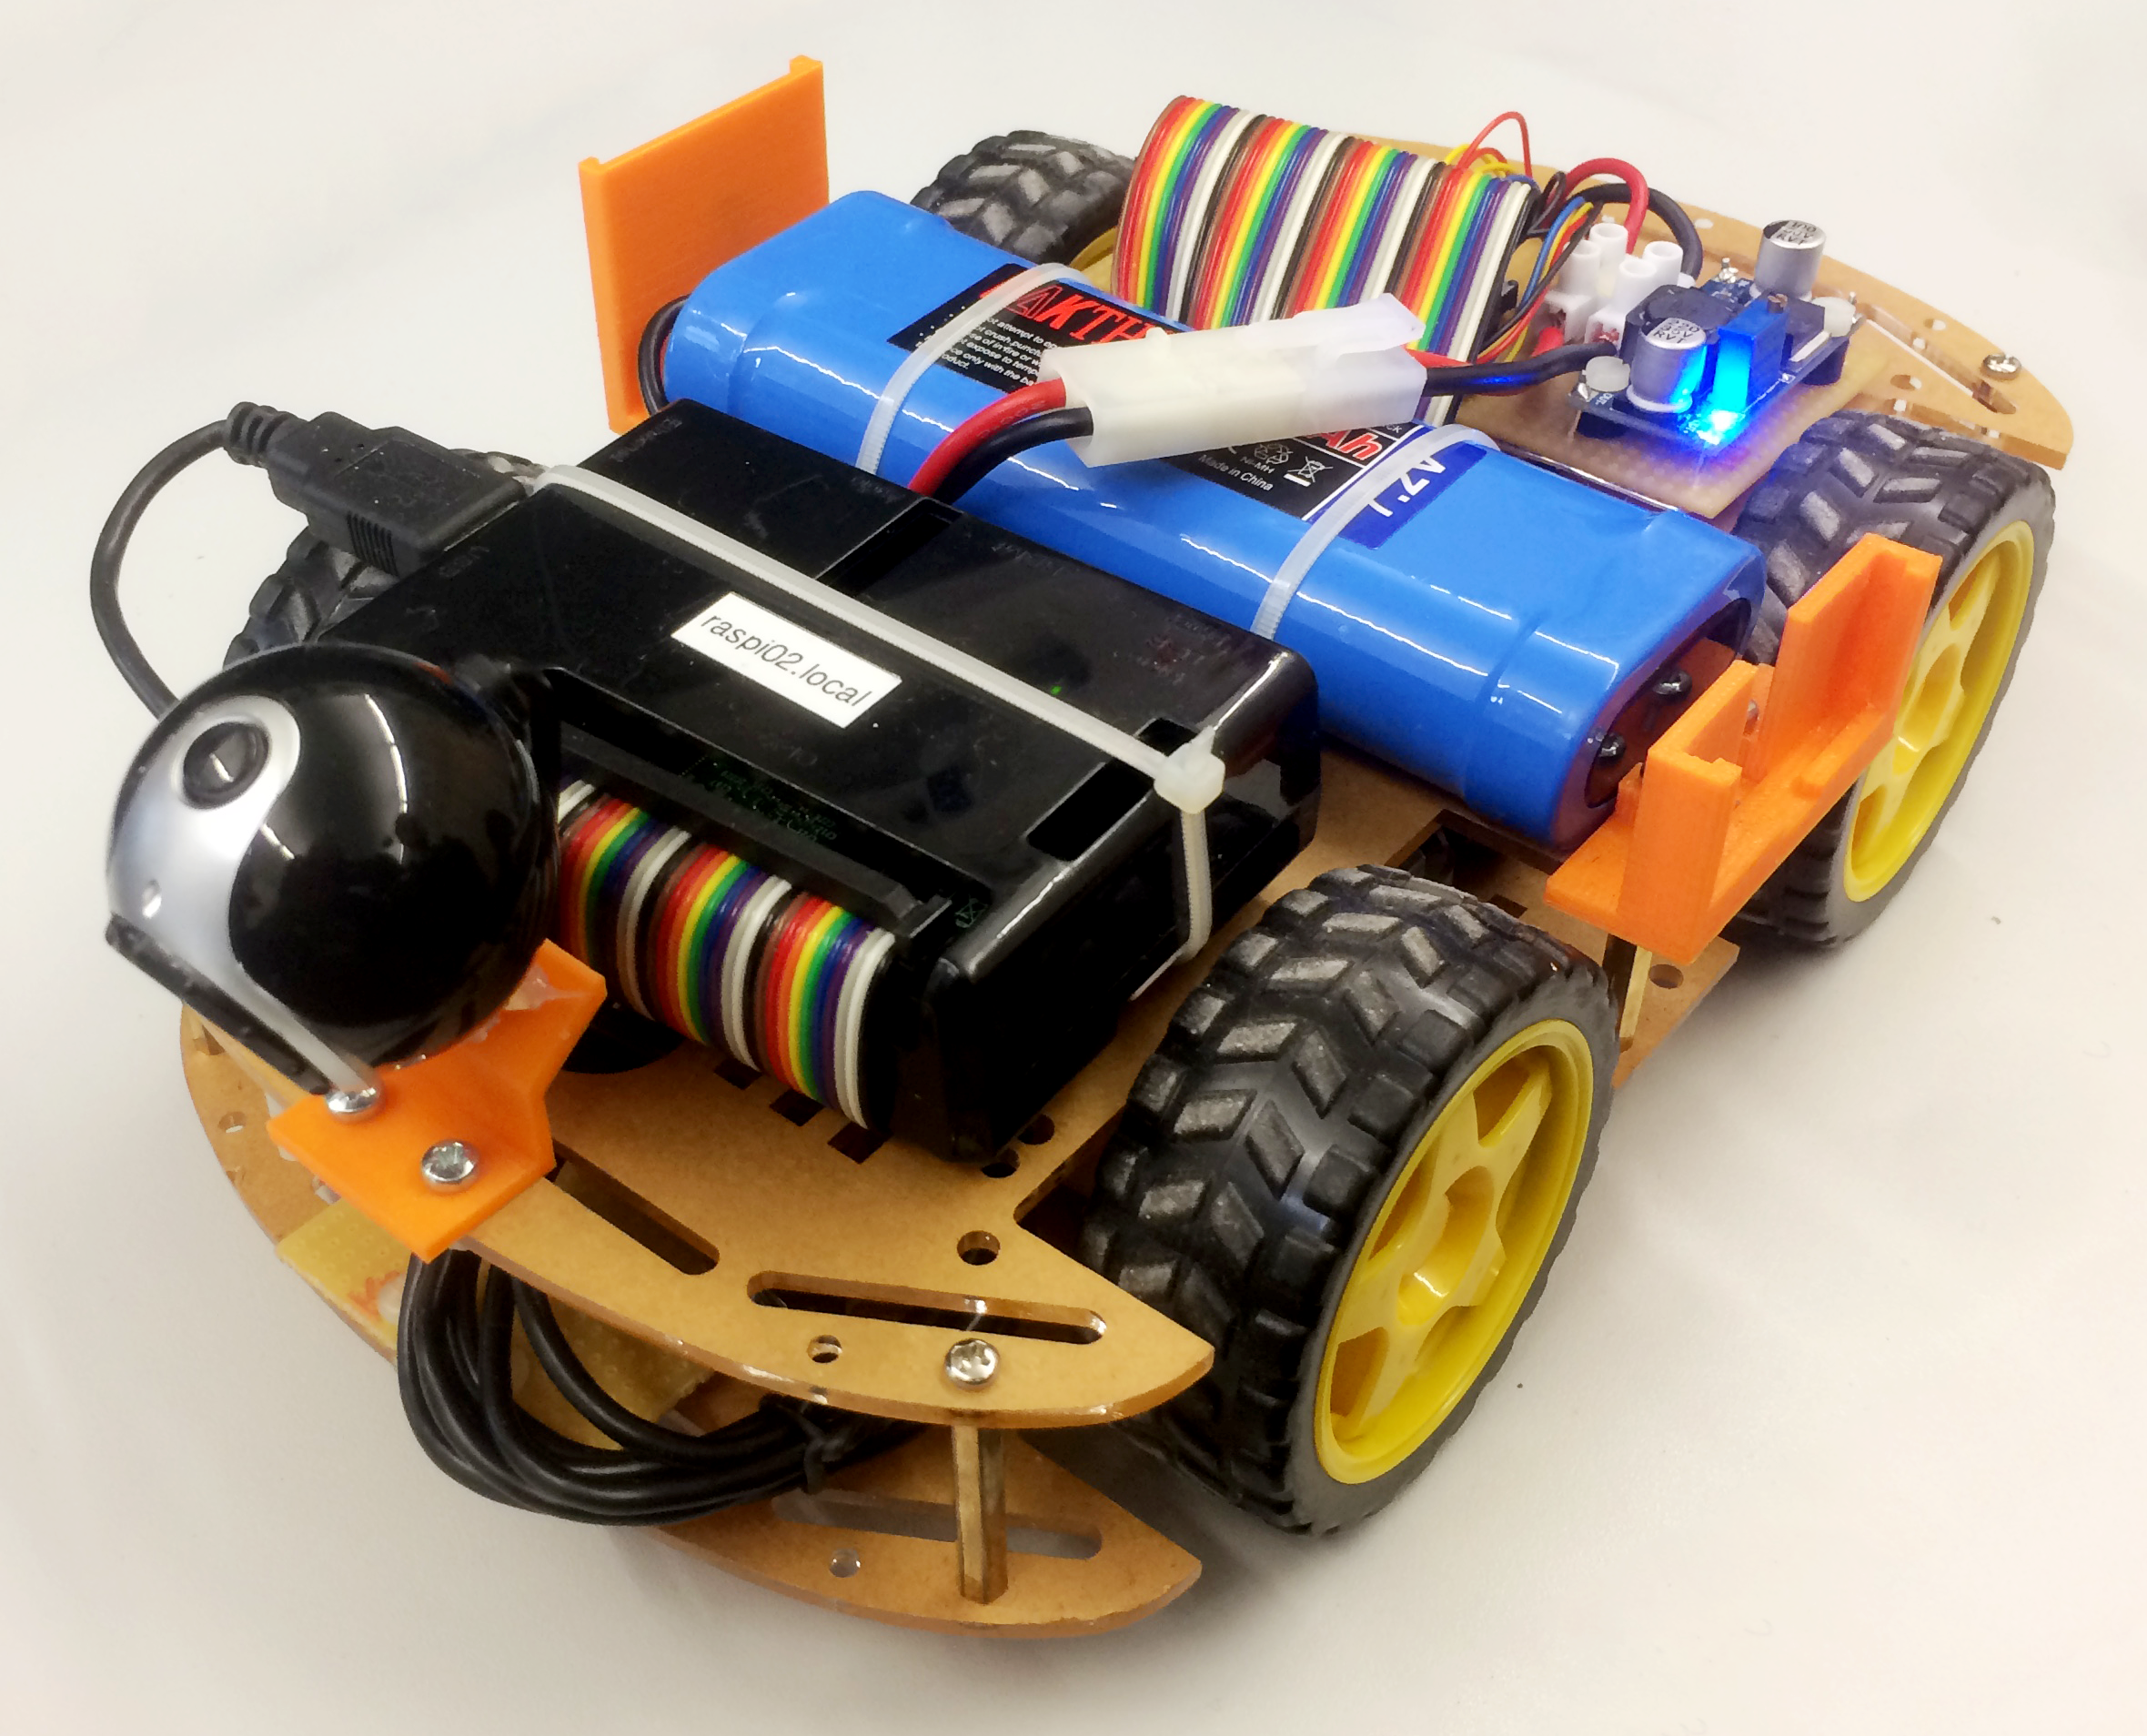
\includegraphics[width=\textwidth]{../bilder_videos/RaspberryCar.png}
	\end{subfigure}%
	\begin{subfigure}{.5\textwidth} \centering
		\includegraphics[width=\textwidth]{../bilder_videos/RaspberryCar-2.png}
	\end{subfigure}%
	\caption{Das Auto im Finalen Aufbau}
	\label{auto}
\end{figure}

\section{Schaltplan}

\begin{figure}[ht!] \centering
	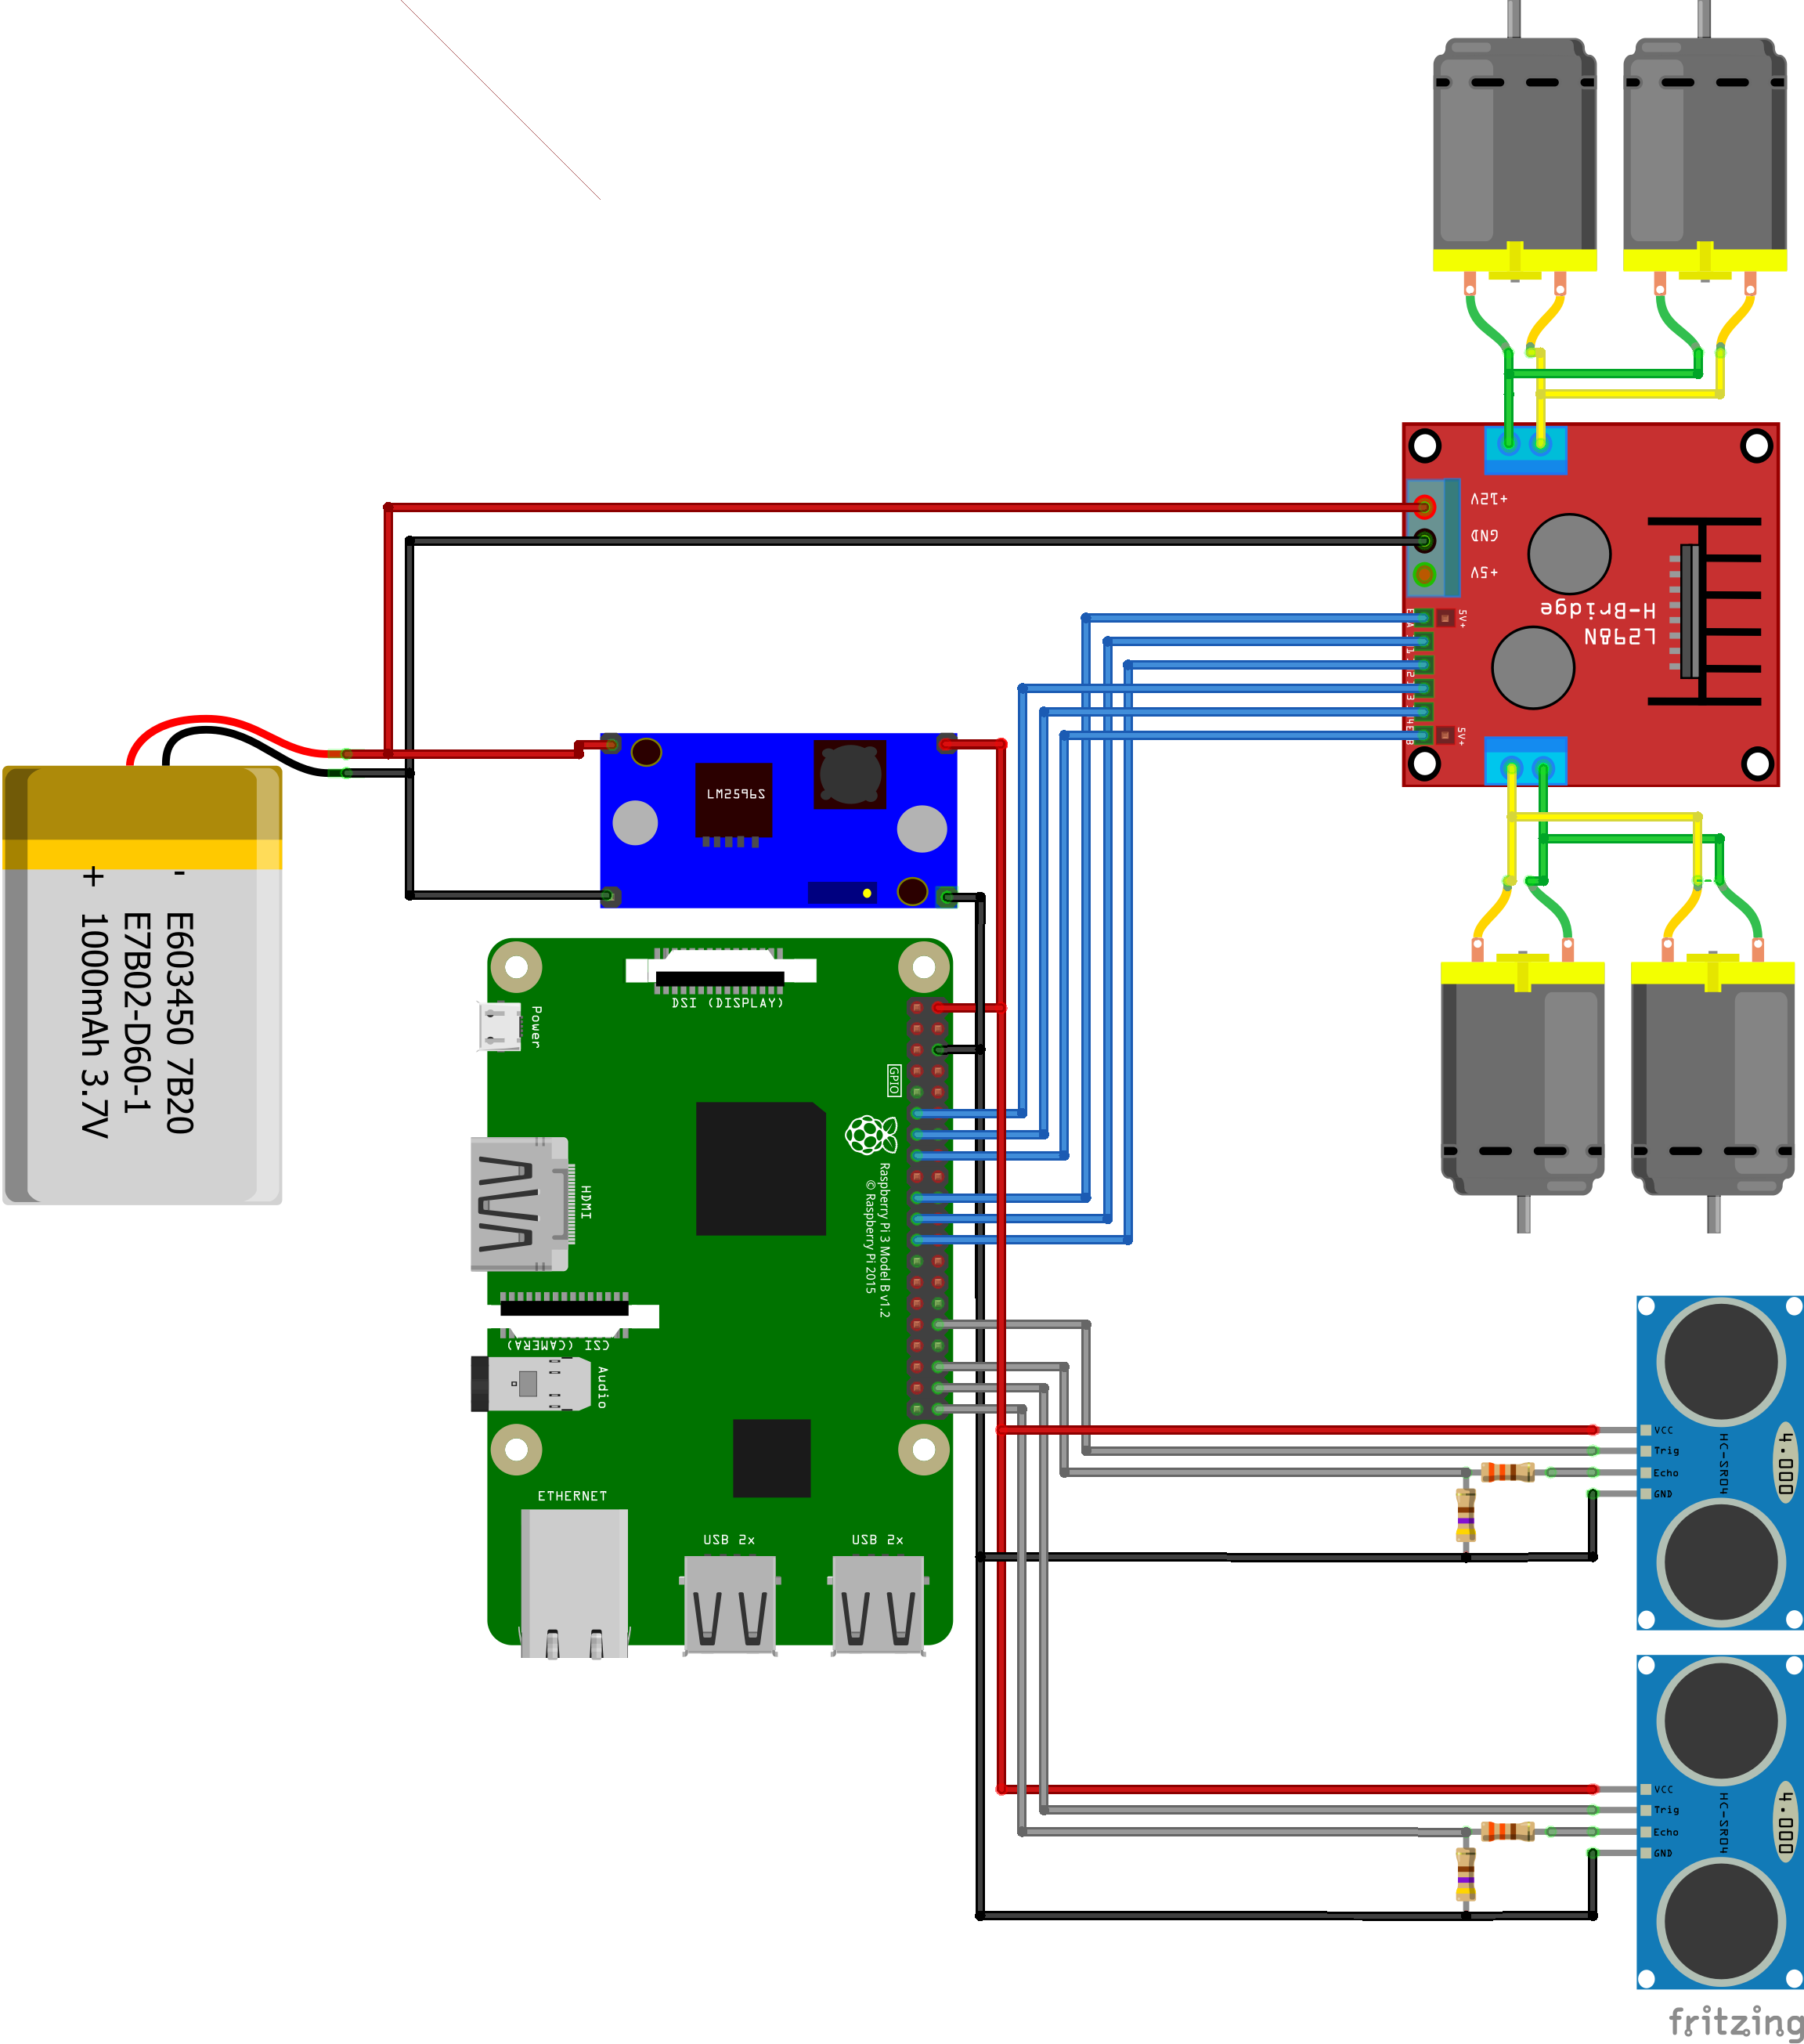
\includegraphics[width=.5\textwidth]{Schaltplan_Steckplatine.png}
	\caption{Schaltplan}
	\label{schaltplan}
\end{figure}

\newpage
\section{Code}

Das Programm wird über die \textit{main.py} Datei ausgeführt. Zwei Module \textit{setup.py} und \textit{aufrauemen.py} sind ausgelagert, dadurch ist die Hauptdatei übersichtlicher und die Module können einfacher von anderen Dateien mitbenutzt werden.

\subsection{main.py}

In \textit{main.py} wird threading verwendet, was gleich mehrere Vorteile hat. Die Bilderaufnahme ist extrem viel schneller, wenn sie auf einem anderen thread als der restliche Algorithmus läuft und das abspeichern der Bilder für eine Videoausgabe würde ohne das threading die Rechendauer um ein vielfaches erhöhen. Außerdem können so andere Funktionen unabhängig von dem restlichen Programm problemlos ausgeführt werden.

Es laufen drei threads parallel. Der eigentliche Fahralgorithmus \textit{linienfahren}, die Videoausgabe \textit{makevideo} und die Ampelüberprüfung \textit{checkblue}. \textit{linienfahren} ruft zwei Funktionen auf, \textit{line} zum Bildaufnehmen und \textit{lenken} zur Motorsteuerung.

Es werden mehrere globale Variablen zwischen den einzelnen threads benutzt. Zum einen die Bildvariablen \textit{ret} und \textit{img}, damit nicht jede Funktion eigene Bilder aufnehmen muss und zum anderen der Linienmesswert \textit{x} und die verstrichene Zeit \textit{minutes, seconds}, die zur Videoausgabe benötigt werden.


\subsubsection{import}	%%%%%%%%%% import %%%%%%%%%%
\lstinputlisting[language=Python,firstline=1,lastline=14]{../main.py}

Am Anfang der Hauptdatei werden die benötigten Module importiert, gefolgt von den beiden ausgelagerten Dateien. Von aufrauemen.py werden die benötigten Funktionen und von setup.py wird alles importiert, da diese Datei keine Funktion enthält.

In den Zeilen $10$ bis $14$ werden die benötigten Einstellungen für OpenCV 2 vorgenommen und ein erstes Bild aufgenommen.

\newpage
\subsubsection{main}	%%%%%%%%%% main %%%%%%%%%%
\lstinputlisting[language=Python,firstline=167]{../main.py}

Das Programm wird in \textit{main} gestartet und beendet. Als erstes werden die Motoren mit der \textit{losfahren} Funktion gestartet, allerdings noch mit einem Tastverhältnis von 0\%.
Anschließend wird das threading gestartet. Dafür wir wird \textit{run\_event}, das als \textit{while}-Bedingung für die threads dient, gesetzt. Die delay-Angaben und die drei verwendeten threads th1, th2 und th3 werden definiert. Dabei ist \textit{target} die Funktion die in dem neuen thread laufen soll und \textit{args} sind die Variablen die mit übergeben werden.
Die drei threads sind \textit{linienfahren} (der eigentliche lenk-Algorithmus), \textit{checkblue} (Test ob die Ampel blau leuchtet) und \textit{makevideo} (die Videoausgabe).\\

Der erste thread (die Videoaufzeichnung) wird gestartet, gefolgt von einer \textit{while}-Schleife die überprüft ob die Ampel grün ist. Wenn der zurückgegebene Wert der \textit{checkgreen} Funktion größer gleich 500 ist, also ausreichend Grünanteile erkannt wurden endet die Schleife. Dadurch werden die anderen beiden threads gestartet, wodurch das Auto losfährt.

Damit das Programm wieder beendet werden kann, folgt eine \textit{try-while} und \textit{except} Schleife, die weiter keine andere Funktion hat. Sobald ein \textit{KeyboardInterrupt} durch das drücken von Strg-c auftritt wird das Auto gebremst und die threads werden geschlossen. Allerdings muss dabei gewartet werden bis die \textit{while}-Schleifen aller threads durchgelaufen sind. Anschließend werden die GPIO einstellungen bereinigt, die Videoaufnahme beendet und das Video gespeichert.\\

Gestartet wird die \textit{main} Funktion durch eine \textit{if \_\_name\_\_ == "\_\_main\_\_"} abfrage, um die Datei auch als Modul verwenden zu können.

\newpage
\subsubsection{line}	%%%%%%%%%% line %%%%%%%%%%
\lstinputlisting[language=Python,firstline=104,lastline=119]{../main.py}

In \textit{line} wird ein Bild aufgenommen und, in einer Zeile, der Mittelpunkt der roten Anteile ermittelt.

Der Funktion wird beim aufrufen die Zeile (\textit{zeileNr}) übergeben, die auf den Rotwert analysiert werden soll. Damit wird es ermöglicht die selbe Funktion zum analysieren unterschiedlicher Zeilen zu verwenden. Das wird in der finalen Version aber nicht benutzt.

In Zeile $12$ bis $16$ wird der Mittelpunkt berechnet und zurückgegeben. Falls kein Rotanteil über dem Schwellwert liegt, wird \textit{None} zurückgegeben.

\newpage
\subsubsection{linienfahren}	%%%%%%%%%% linienfahren %%%%%%%%%%
\lstinputlisting[language=Python,firstline=122,lastline=164]{../main.py}

\textit{linienfahren} ruft die Funktion \textit{line} auf und berechnet die Lenkung und Geschwindigkeit aus dem zurückgegebenen Wert.

Am Anfang der Funktion wird ein Testbild aufgenommen und die für die Berechnung benötigten Variablen erstellt. Danach folgt eine \textit{while} Schleife, die bis zum Beenden des threading durchläuft.
Falls keine rote Linie im Bild war, oder in seltenen Fällen, wenn die Linie nicht erkannt wurde, gibt \textit{line} \textit{None} zurück. In diesem Fall wird, in den Zeilen $17$ bis $21$, überprüft ob die Linie zuletzt rechts oder links im Bild war. Der Messwert \textit{mitte} wird dementsprechend auf das Minimum (0) oder das Maximum (640) gesetzt. Anschließend wird der Wert für die Videoausgabe abgespeichert (Zeile $22$).

In den Zeilen $24$ bis $33$ wird der Wert für die Lenkung und Geschwindigkeit berechnet. Unterschieden wird zwischen drei Fällen. Ist der Messwert in der Mitte des Bildes wird geradeaus gelenkt, andernfalls wird die Lenkung und die Geschwindigkeit berechnet. Ist der Messwert größer als der Bildmittelpunkt wird $2-\textit{Lenkwert}$ gerechnet. Es ergibt sich ein Lenkwert zwischen 0 und 1 für eine Linkskurve und 1 bis 2 für eine Rechtskurve. Das hat den Vorteil, dass der \textit{lenken} Funktion nicht zusätzlich eine Richtungsangabe übergeben werden muss. Anschließend wird die \textit{lenken} Funktion mit den Lenk- und Geschwindigkeits-Variablen aufgerufen .\\

Der Wert für die Lenkung und die Geschwindigkeit wird aus dem Messwert und dem Bildmittelpunkt berechnet:
\begin{align}
	\text{Lenkung}&=\dfrac{\text{Messwert}}{\text{Bildmittelpunkt}}\cdot 90\% + 10\% \\
	\text{Geschwidigkeit}&=\dfrac{\text{Messwert}}{\text{Bildmittelpunkt}}\cdot 60\% + 40\%
\end{align}
Damit die Lenkung nicht zu stark ist, wird der Wert kleiner gewichtet ($\cdot 90\%$) und angehoben ($+10\%$). So startet der Wert nicht bei 0\% sondern bei 10\%.
Die Geschwindigkeit wird gleich berechnet, allerdings mit ($\cdot 60\%$) gewichtet und ($+40\%$) angehoben. Es wird also mit 60\% bis 100\% Geschwindigkeit gefahren.\\

Für die Text- und Videoausgabe wird die verstrichene Zeit berechnet.
Anschließend folgt in Zeile $40/41$ eine Textausgabe über die Konsole. Dabei werden $\frac{\textit{Messwert}}{10}$ Leerzeichen, dann ein Blockzeichen als Position des Messpunktes im Bild und die verbleibenden $64-\frac{\textit{Messwert}}{10}$ Leerzeichen geschrieben. Dann folgen noch Angaben zu Messpunkt, Lenkwert, Geschwindigkeit und Zeit. In der nächsten Zeile wird der Mittelpunkt mit einem Strich markiert. Es ergibt sich eine Textausgabe die zum Beispiel so aussieht:

\begin{lstlisting}[language=bash,basicstyle=\tiny,numbers=none]
               █                               x = 245.0 ;steer = 0.8 ;speed = 85.9 ;time = 00:00.00
                       |
                 █                             x = 265.0 ;steer = 0.8 ;speed = 89.7 ;time = 00:00.04
                       |
                   █                           x = 284.0 ;steer = 0.9 ;speed = 93.2 ;time = 00:00.08
                       |
                    █                          x = 292.0 ;steer = 0.9 ;speed = 94.8 ;time = 00:00.12
                       |
                     █                         x = 304.0 ;steer = 1.0 ;speed = 97.0 ;time = 00:00.16
                       |
                      █                        x = 312.0 ;steer = 1.0 ;speed = 98.5 ;time = 00:00.20
                       |
                       █                       x = 325.0 ;steer = 1.0 ;speed = 99.1 ;time = 00:00.24
                       |
\end{lstlisting}

\newpage
\subsubsection{lenken}	%%%%%%%%%% lenken %%%%%%%%%%
\lstinputlisting[language=Python,firstline=76,lastline=101]{../main.py}

Die \textit{lenken} Funktion steuert das Tastverhältnis der Motoren. Übergeben werden zwei Parameter für die Lenkgewichtung und die Geschwindigkeit.
Am Anfang der Funktion werden einige Abfragen zur Fehlerverhütung vorgenommen, damit das Tastverhältnis nicht unter 0\% oder über 100\% liegt, dass würde sonst zu einem Absturz führen.\\
Damit das Auto in den Kurven nicht ungewollt langsamer fährt, wird ausgerechnet wie viel schneller sich die äußeren  Motoren drehen können.
\begin{align}
	\text{Kopfraum} = 100-\text{Geschwindigkeit}
\end{align}
Ist der Kopfraum größer als der Geschwindigkeitswert, wird der Kopfraum gleich der Geschwindigkeit gesetzt.\\

Die Tastverhältnisse der Motoren werden gleich dem Geschwindigkeitswert gesetzt, wenn der Lenkwert $steer=1$ ist. Sonst wird unterschieden ob der Lenkwert größer oder kleiner als 1 ist, um in die entsprechende Richtung zu lenken.
\begin{align}
	&\text{Innere Motoren:} &\text{Tastverhältnis} &= \text{Lenkwert}\cdot\text{Geschwindigkeit}\\
	&\text{Äußere Motoren:} &\text{Tastverhältnis} &= (1-\text{Lenkwert})\cdot\text{Kopfraum}+\text{Geschwindigkeit}
\end{align}
Die Kombination aus dem Lenkwert, Geschwindigkeitswert und Kopfraum ermöglicht ein stufenloses kurven fahren, ohne das an Geschwindigkeit verloren wird. Dabei ist es egal worauf die Werte basieren, es wird immer gleich sanft gelenkt.

\begin{table}[th!]
	\centering
	\caption{Beispielwerte für die Motorensteuerung}
	\begin{tabular}{c|c|c|c}
		Lenken & Geschwindigkeit & $T_{\text{innen}} [\%]$ &  $T_{\text{au\ss en}}[\%]$ \\ \hline 
		0,2 & 20 & \ 2 & 36 \\  
		    & 60 & 12  & 92 \\    
		    & 80 & 16  & 96 \\ \hline
		0,8 & 20 & 16  & 24 \\
		    & 60 & 48  & 68 \\
		    & 80 & 64  & 84 \\
	\end{tabular} 
\end{table}

\newpage
\subsubsection{checkgreen}	%%%%%%%%%% checkgreen %%%%%%%%%%
\lstinputlisting[language=Python,firstline=36,lastline=50]{../main.py}

Die \textit{checkgreen} Funktion Analysiert ein ganzes Bild der Webcam auf ihren Grünanteil und gibt die Anzahl zurück.

\newpage
\subsubsection{checkblue}	%%%%%%%%%% checkblue %%%%%%%%%%
\lstinputlisting[language=Python,firstline=53,lastline=73]{../main.py}

\textit{checkblue} funktioniert ähnlich wie \textit{checkgreen}, allerdings läuft die Funktion in Dauerschleife und stoppt das Auto 1,5 Sekunden nachdem die blaue Ampel erkannt wurde.
Die Funktion nimmt dabei kein eigenes Bild auf, sondern verwendet das Bild, dass von der \textit{linienfahren} Funktion aufgenommen wurde. Beim starten des threads wartet die Funktion eine Sekunde, damit die grüne Ampel nicht fälschlicher weise als Stopsignal erkannt wird.

\newpage
\subsubsection{makevideo}	%%%%%%%%%% mekvideo %%%%%%%%%%
\lstinputlisting[language=Python,firstline=17,lastline=33]{../main.py}

Die Aufgabe der \textit{makevideo} Funktion ist es die von der Kamera aufgenommenen Bilder als ein Video zu exportieren. Da das Video nur zur Fehleranalyse und Veranschaulichung dient, wird es vernachlässigt ob das Video in Echtzeit läuft. Dafür wird die aktuelle Fahrzeit, ab dem erkennen der grünen Ampel, unten links im Bild eingeblendet. Außerdem wird der zu dem Bild gehörende Messpunkt und dessen Wert eingezeichnet.

Das Video in Zusammenhang mit den eingeblendeten Werten ermöglicht eine deutlich bessere Fehleranalyse als eine Textausgabe über die Konsole (Abb.: \ref{schuh_im_bild}).

\begin{figure}[ht!] \centering
	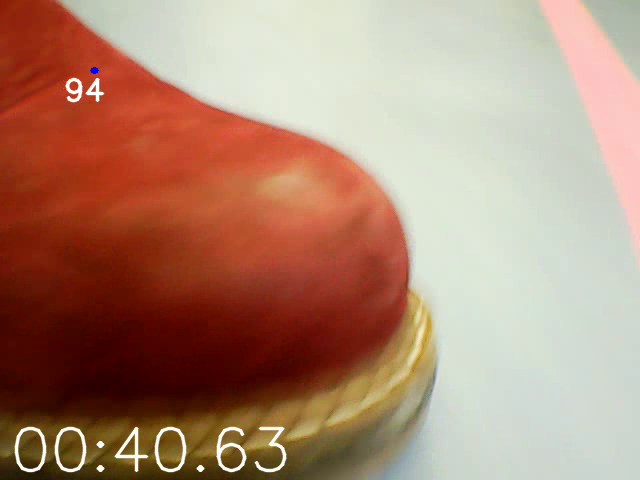
\includegraphics[width=.5\textwidth]{schuh_im_bild.png}
	\caption{Kamerabild mit Zeitanzeige und Messpunkt, abgelenkt von einem roten Schuh}
	\label{schuh_im_bild}
\end{figure}

\newpage
\subsection{setup.py}	%%%%%%%%%% setup %%%%%%%%%%
\lstinputlisting[language=Python]{../setup.py}

In \textit{setup.py} werden die GPIOs definiert, der Skript wird am Anfang von \textit{main.py} aufgerufen. Verwendet wird der BCM Modus. Für die PWM wurde eine Frequenz von $\unit[73]{Hz}$ gewählt.

Dadurch dass das GPIO-Setup ausgelagert war konnten alle Python Skripte während der ganzen Entwicklungsphase problemlos verwendet werden. Wenn die GPIOs sich ändern, muss dies nur in dieser einen Datei eingetragen werden.

\newpage
\subsection{aufraeumen.py}	%%%%%%%%%% aufräumen %%%%%%%%%%
\lstinputlisting[language=Python]{../aufraeumen.py}

In \textit{aufrauemen.py} sind drei Funktionen ausgelagert. \textit{losfahren} setzt die vier GPIOs der Motoren auf die entsprechenden Werte zum Vorwärtsfahren, \textit{bremsen} setzt die GPIOs, zum stoppen des Autos, auf null und \textit{aufrauemen} stoppt das Auto und bereinigt die GPIO Einstellungen.


\newpage
\section{3D-Druck Halterungen}

\subsection{Kamerahalterung}
\begin{figure}[ht!] \centering
	\begin{subfigure}{.33\textwidth} \centering
		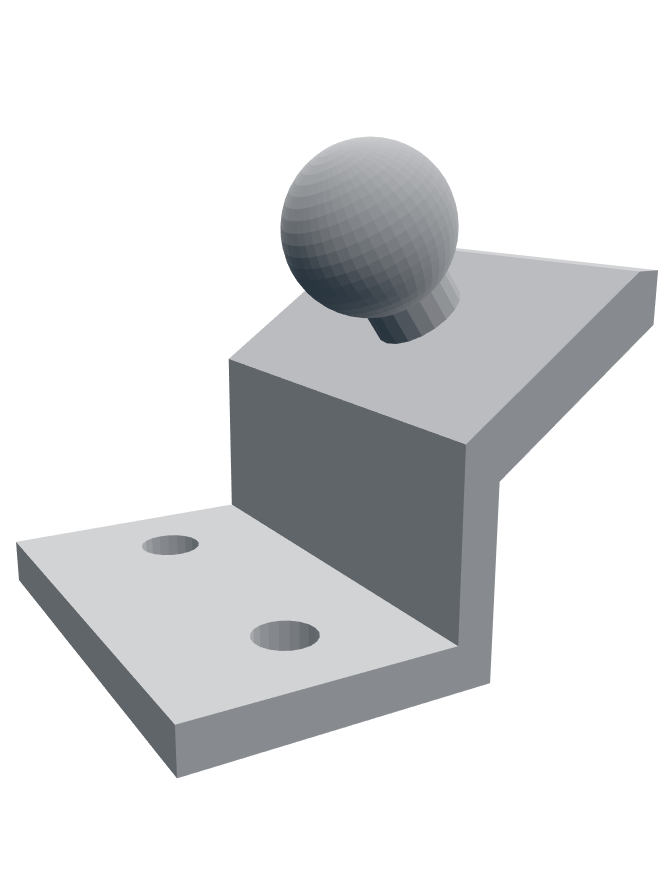
\includegraphics[width=\textwidth]{../3D-Druck_Modelle/Kamerahalterung_neu.png}
	\end{subfigure}%
	\begin{subfigure}{.33\textwidth} \centering
		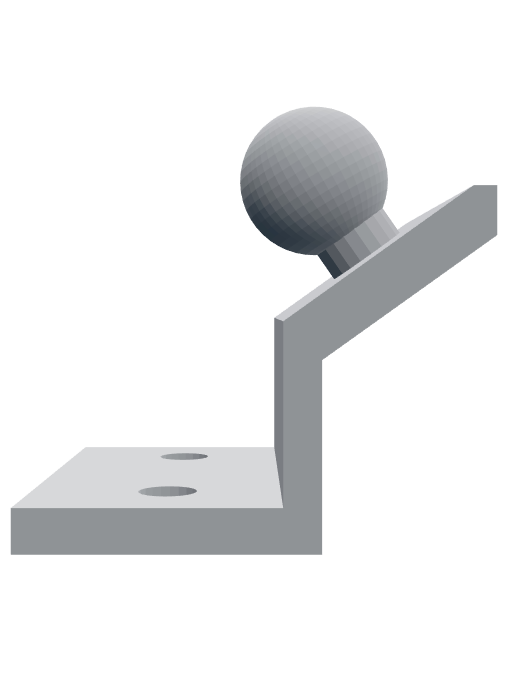
\includegraphics[width=\textwidth]{../3D-Druck_Modelle/Kamerahalterung_neu_top.png}
	\end{subfigure}%
	\begin{subfigure}{.33\textwidth} \centering
		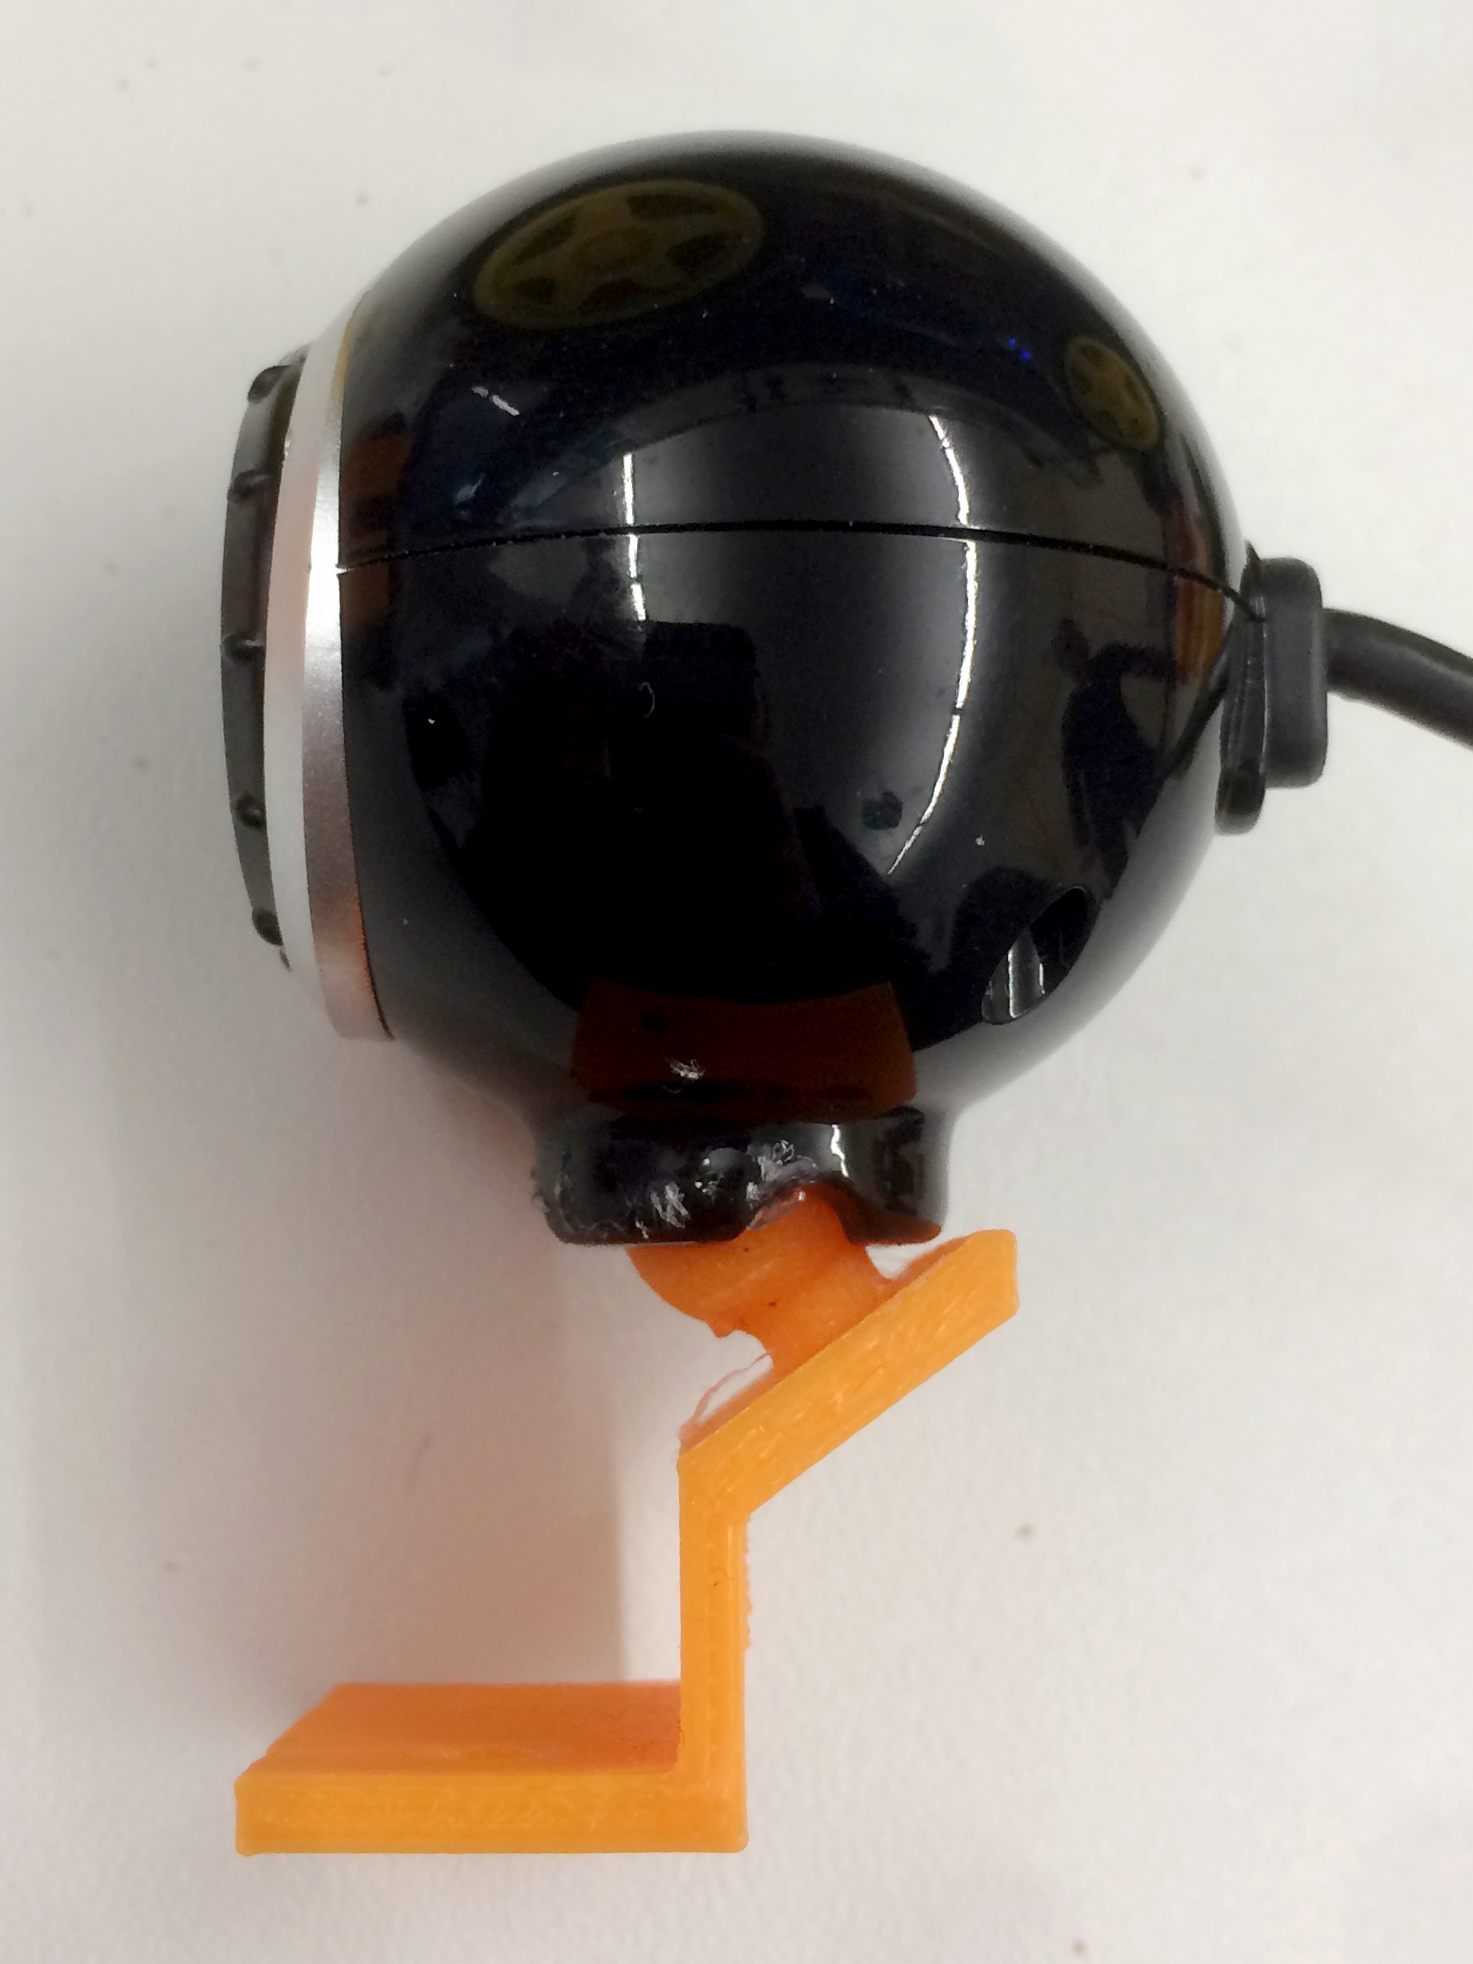
\includegraphics[width=\textwidth]{../bilder_videos/Kamerahalterung.png}
	\end{subfigure}%
	\caption{Kamerahalterung 3D-Modell und fertiger 3D-Druck}
	\label{kamerahalterung}
\end{figure}

\begin{figure}[ht!] \centering
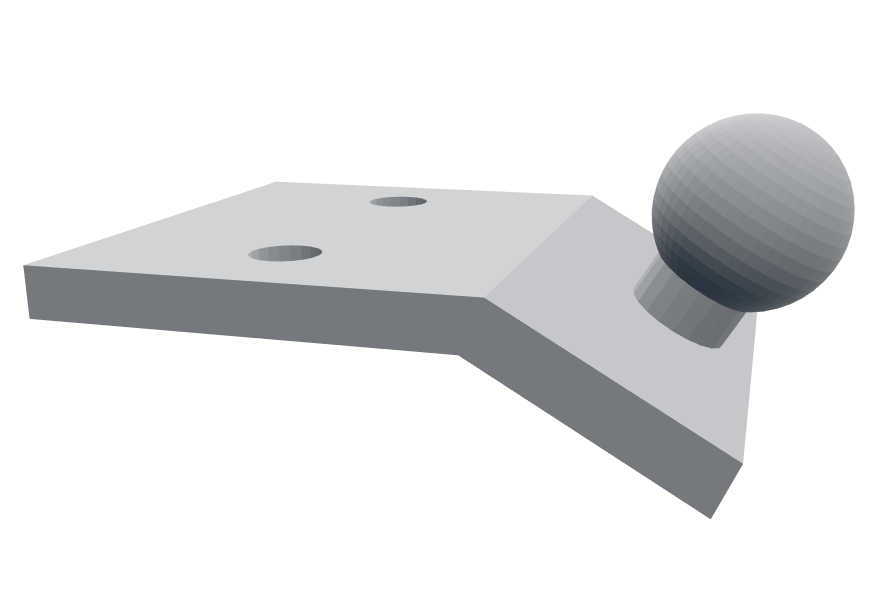
\includegraphics[width=.5\textwidth]{../3D-Druck_Modelle/Kamerahalterung_alt.png}
\caption{3D-Modell der ersten Kamerahalterung}
\label{kamerahalterung alt}
\end{figure}

\subsection{Ultraschallsensorhalterung}

Für den Ultraschallsensor HC-SR04 wurde eine Halterung entworfen die es ermöglicht den Sensor sowohl aufrecht als auch Kopfüber an dem Auto zu befestigen. Außerdem sollte der Sensor, wie alle Teile des Autos einfach abnehmbar sein, falls Änderungen vorgenommen werden müssen. Entworfen wurde das Modell in Blender 2.79, mit zwei löchern für Schrauben, platz für weitere Bohrungen und einen Schlitz für die Steckverbindung.

Der 3D-Druck ging problemlos und die Halterung erfüllte die Anforderungen, es stellte sich aber heraus, dass die Maße der Sensoren teilweise zu stark voneinander abweichen, deswegen wurde das Modell noch einmal mit mehr Spielraum überarbeitet.

\begin{figure}[ht!] \centering
	\begin{subfigure}{.5\textwidth} \centering
		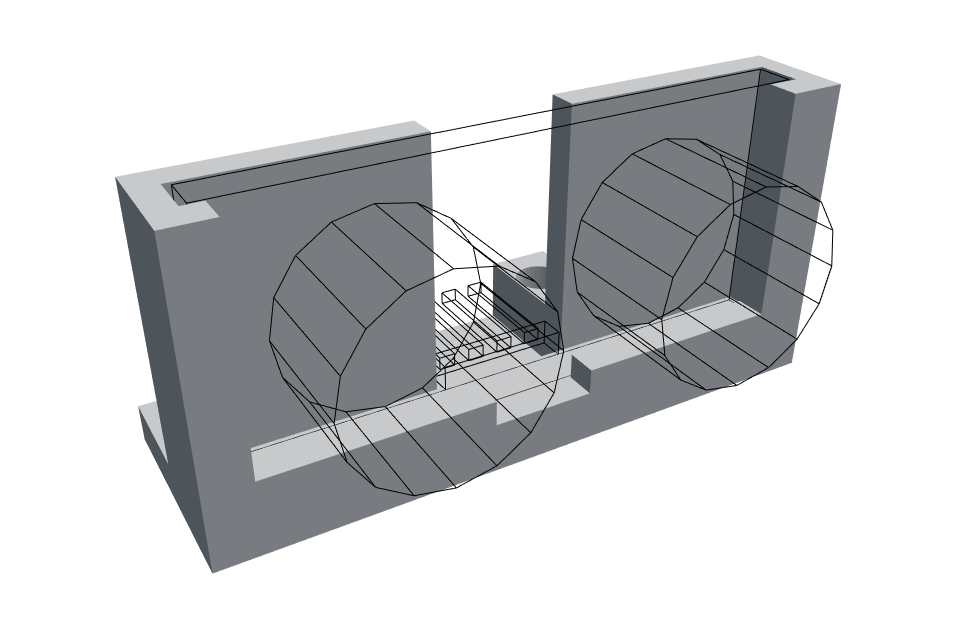
\includegraphics[width=\textwidth]{../3D-Druck_Modelle/Sensorhalterung.png}
	\end{subfigure}%
	\begin{subfigure}{.5\textwidth} \centering
		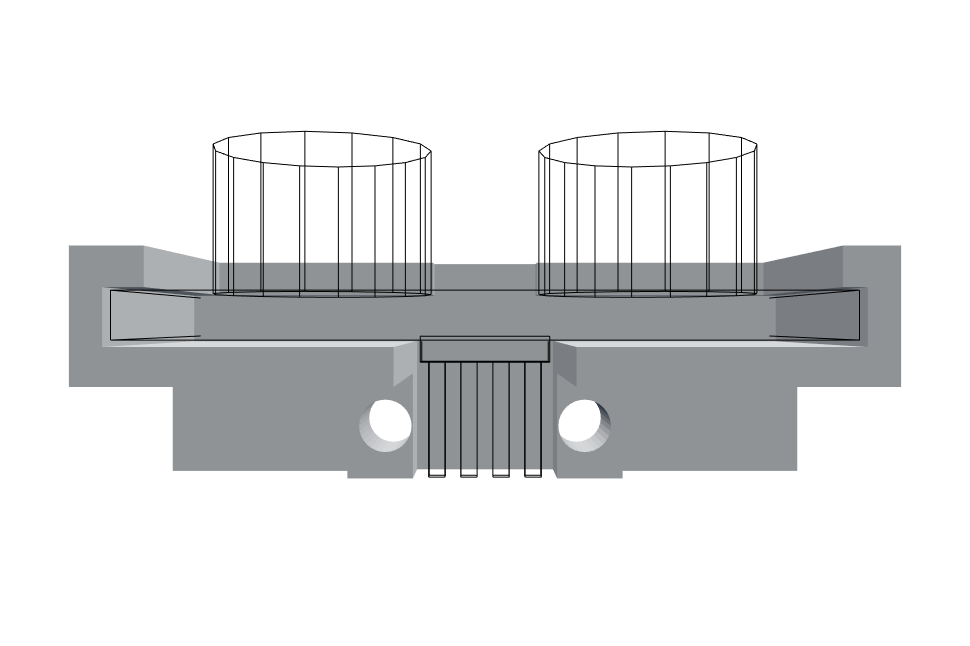
\includegraphics[width=\textwidth]{../3D-Druck_Modelle/Sensorhalterung_Top.png}
	\end{subfigure}\\
	\begin{subfigure}{.5\textwidth} \centering
		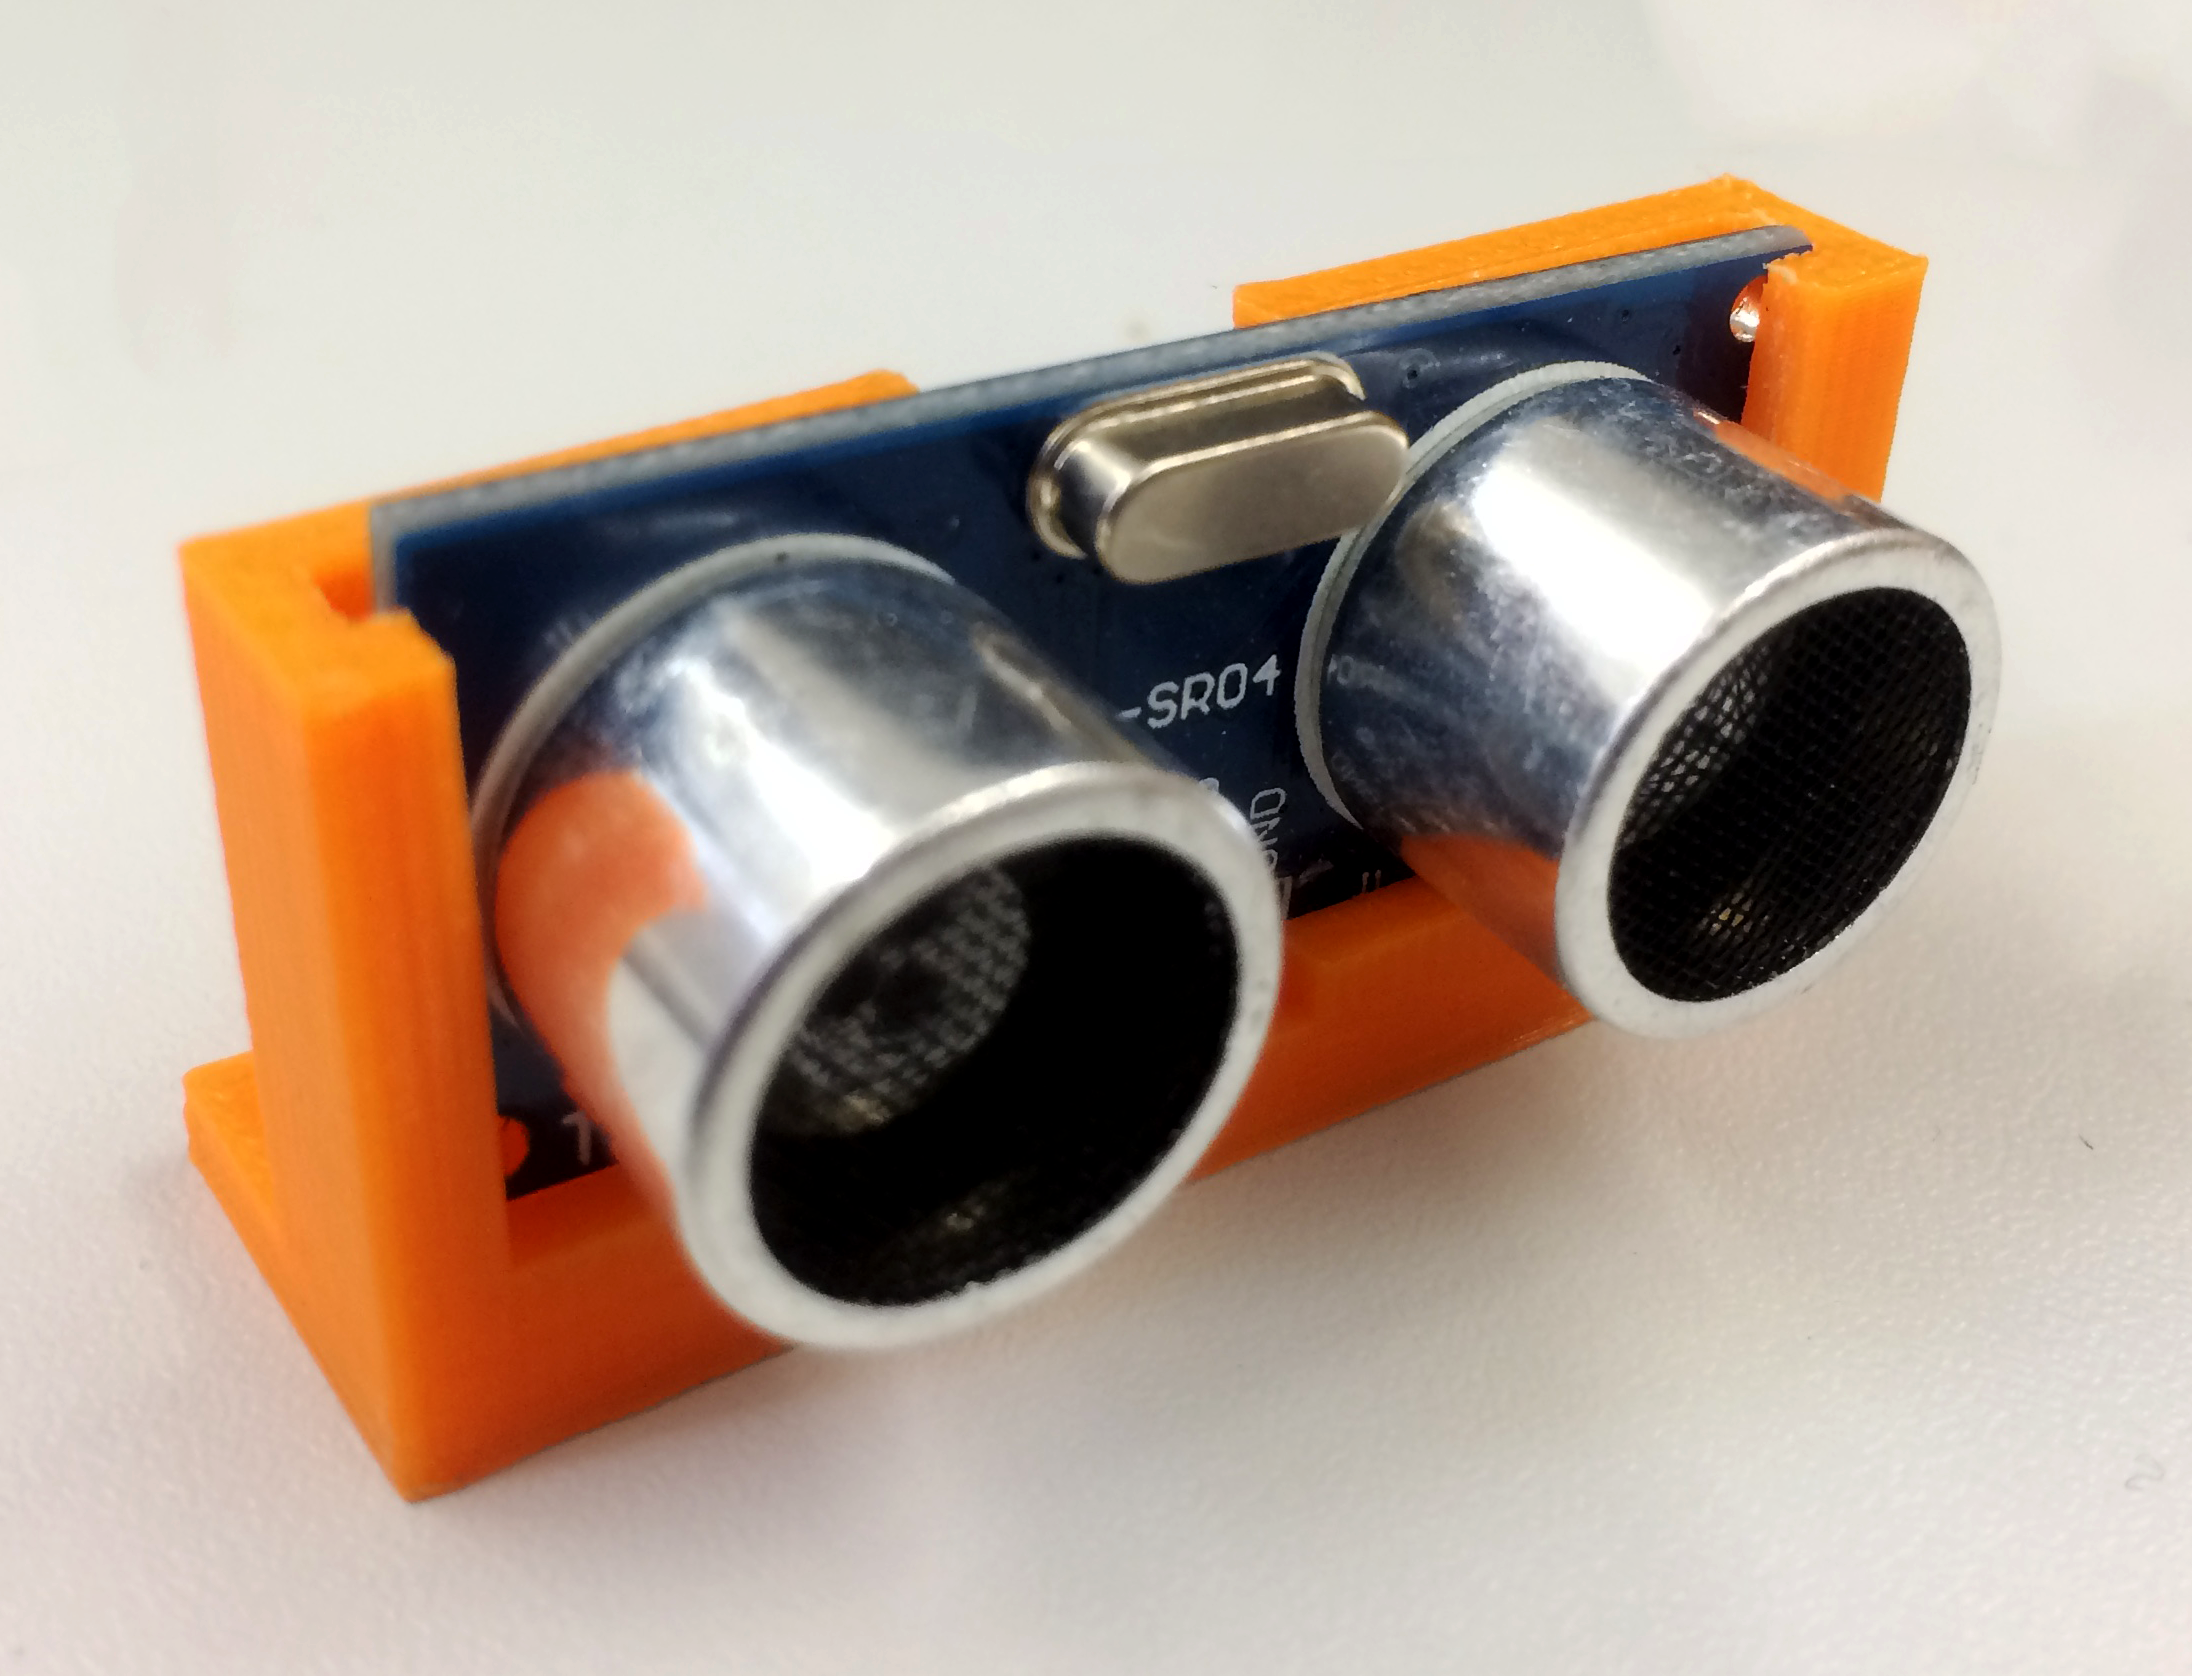
\includegraphics[width=\textwidth]{../bilder_videos/Sensorhalterung.png}
	\end{subfigure}%
	\begin{subfigure}{.5\textwidth} \centering
		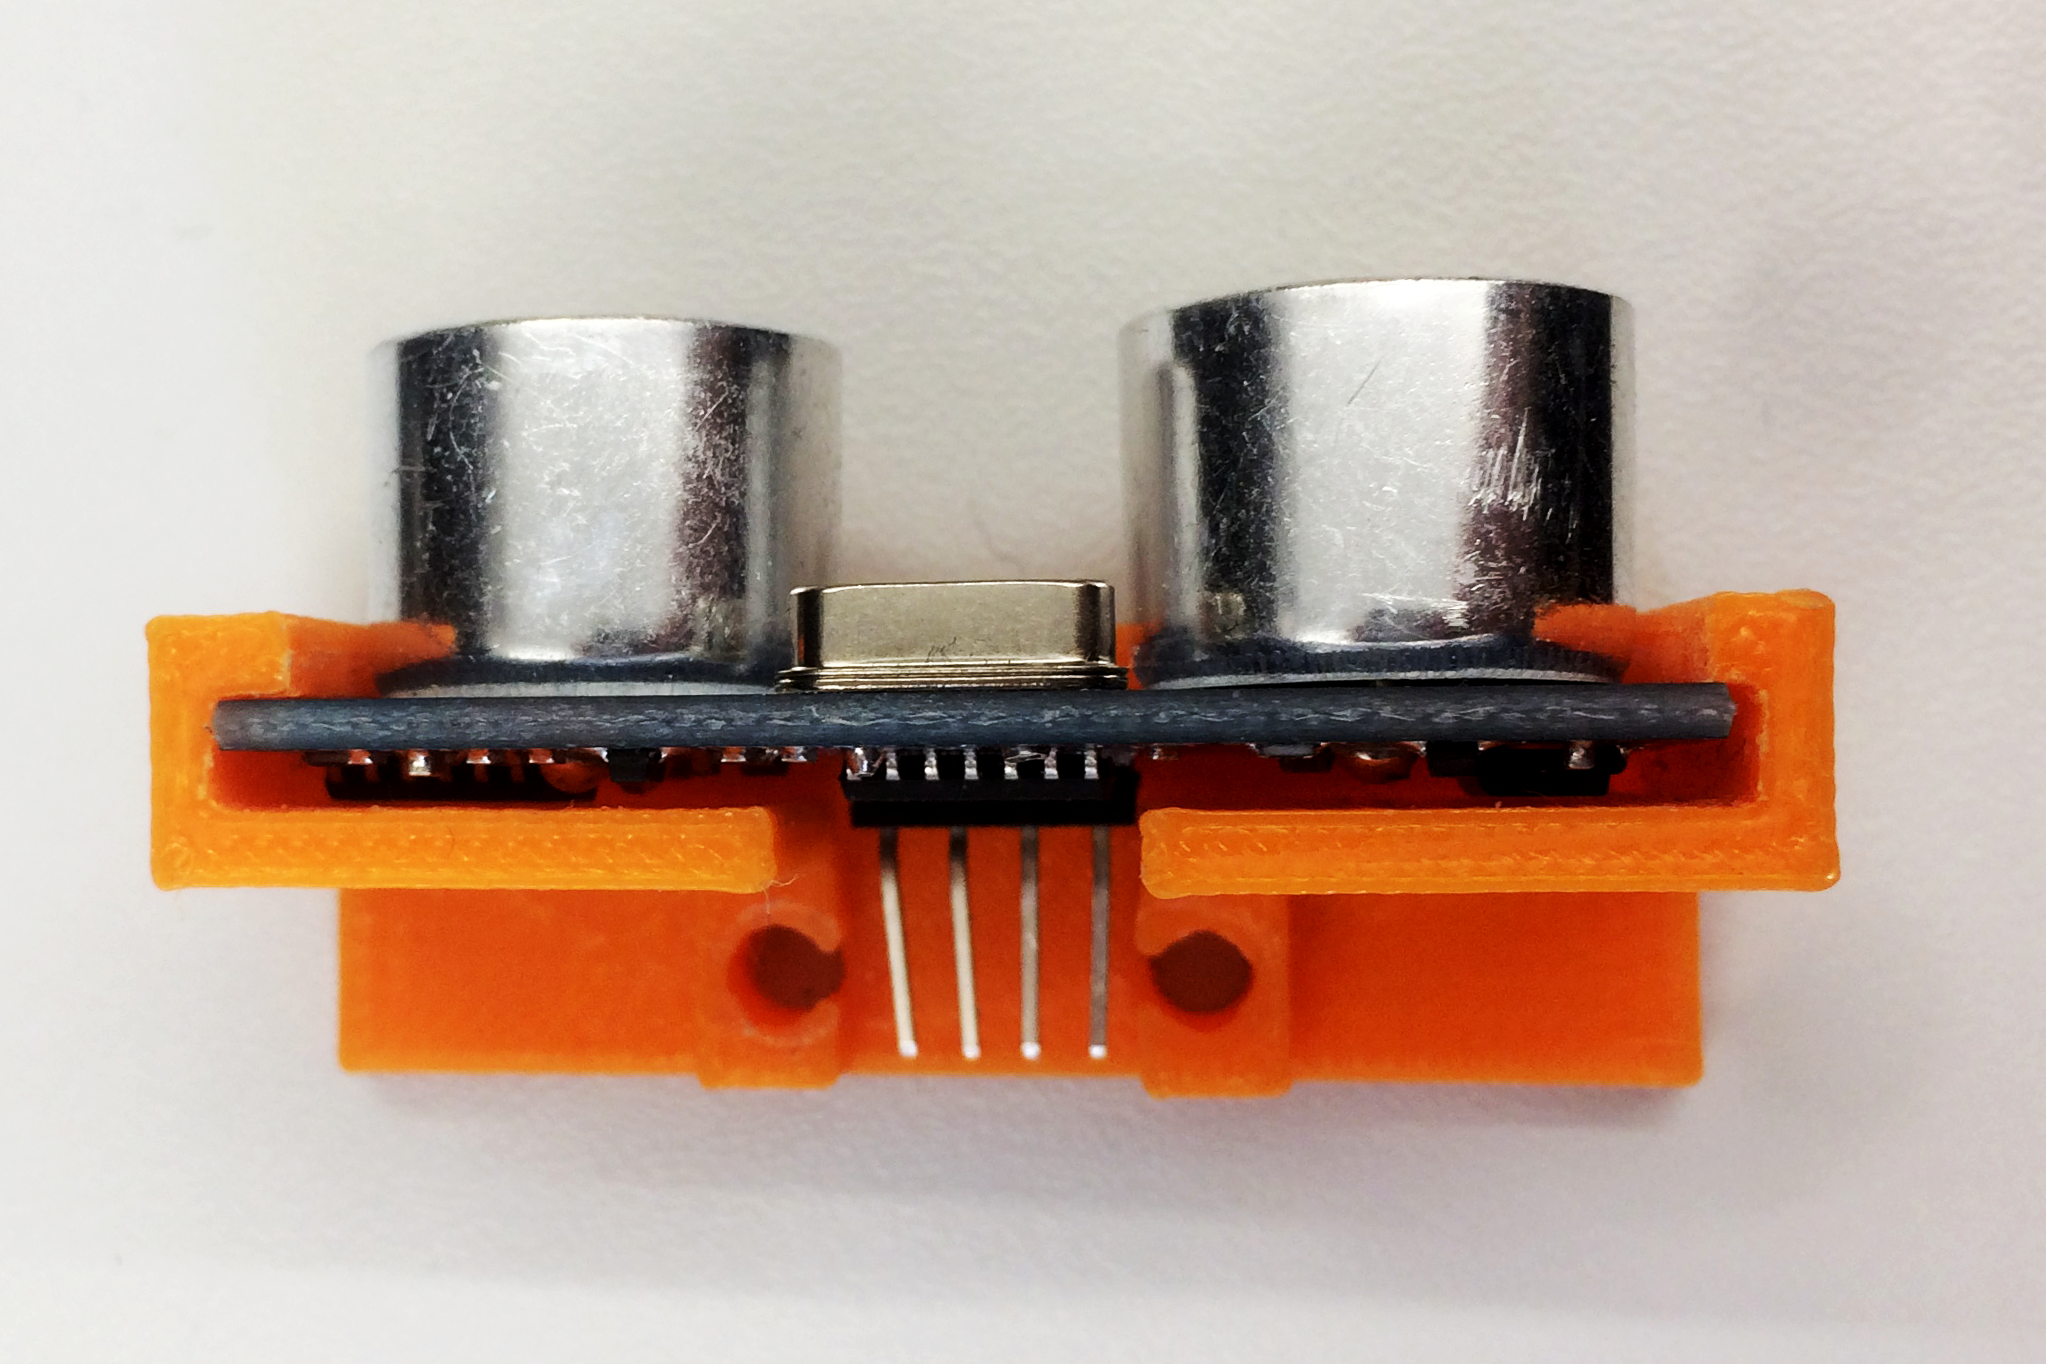
\includegraphics[width=\textwidth]{../bilder_videos/Sensorhalterung_Top.png}
	\end{subfigure}%
	\caption{Ultraschallsensorhalterung 3D-Modell und fertiger 3D-Druck}
\end{figure}

\newpage
\section{Geplante Weiterentwicklungen}

Es sind diverse Weiterentwicklungen an dem Auto geplant, die bisher nicht verwirklicht wurden.
Ein Plan ist es die Videoausgabe deutlich auszubauen. So können mehr Messwerte angezeigt werden, wie zum Beispiel die Lenk- und Geschwindigkeitswerte oder die Drehzahl der Motoren und damit die Zurückgelegte Strecke. Optimal wäre die Ausgabe eines Livestreams, was allerdings nur möglich ist, wenn dadurch der Fahralgorithmus nicht verlangsamt wird.
Zudem war eine anzeige der aktuellen Messwerte über LEDs in Entwicklung.

Der Aufbau der Bauteile auf dem Auto soll noch kompakter werden, in dem Platzsparender gelötet wird. Dadurch wären alle Platinen auf der unteren Platte platziert, so dass nur noch der Raspberry Pi, der Akku und die Kamera zu sehen sind.

\newpage
\section{Anhang}

\subsection{main.py}
\lstinputlisting[language=Python]{../main.py}


\end{document}
